% Generic APS style: this REVTeX bundle has no dedicated PRResearch option.
\documentclass[aps,10pt,onecolumn,superscriptaddress,nofootinbib,longbibliography,
  amsmath,amssymb,floatfix]{revtex4-2}
\usepackage[T1]{fontenc}
\usepackage{graphicx}
\usepackage{placeins}
\usepackage{hyperref}
\hypersetup{hidelinks}
% APS BibTeX control includes article titles without a numbered citation.
\makeatletter
\AtBeginDocument{\immediate\write\@auxout{\string\citation{apsrev42Control}}}
\makeatother
\newcommand{\Tr}{\operatorname{tr}}
\newcommand{\Gmax}{G_{\max}^{(2)}}
\newcommand{\Cnoise}{\mathcal C}
\newcommand{\dd}{\mathrm{d}}

\begin{document}
\title{The Stronger Route Can Be the Worse Readout: Flexible Routing under a Fluctuation Budget}
\author{Mingyi Huang}
\affiliation{Research Institute of Intelligent and Complex Systems, State Key
Laboratory of Medical Neurobiology and MOE Frontiers Center for Brain Science,
and Institute of Science and Technology for Brain-Inspired Intelligence,
Fudan University, Shanghai 200433, China}
\affiliation{Shanghai Artificial Intelligence Laboratory, Shanghai 200232, China}
\author{Yuguo Yu}
\email{yuyuguo@fudan.edu.cn}
\affiliation{Research Institute of Intelligent and Complex Systems, State Key
Laboratory of Medical Neurobiology and MOE Frontiers Center for Brain Science,
and Institute of Science and Technology for Brain-Inspired Intelligence,
Fudan University, Shanghai 200433, China}
\affiliation{Shanghai Artificial Intelligence Laboratory, Shanghai 200232, China}

\begin{abstract}
Flexible neural routing must make a cue reliably distinguishable,
not merely produce a large response. We show that two pathways
with fixed gains and proportional mean responses can exchange
discrimination rank as the receiver's integration time changes.
The mechanism is the different persistence of noise entering the
outputs locally, rather than a change in signal timing. When
signal, propagated-noise and cost coefficients are matched, a budget ratio
between the instantaneous and zero-frequency local-noise ratios
guarantees a reversal. We connect this prediction to resource
allocation by deriving exact fluctuation-cost laws for one-way
adjustable couplings with stable internal recurrence. The resulting
noise prices and discrimination ceilings predict gain allocations
that agree with direct optimization in heterogeneous recurrent
modules. Protecting separately required outputs equalizes their
reliability, whereas combining independent outputs balances marginal
benefits. In the controlled two-pathway example, integration time
reverses the direction of budget transfer that improves the worse
output. A distributed feedback model uses downstream errors and
local activity to adjust gains toward the allocation that protects
the weaker output. Thus the computational return on a routing budget depends
on noise location, integration time and the receiver's task, even
when the decay spectrum is fixed.
\end{abstract}
\maketitle

\section{Introduction}

Flexible neural routing allows the same sensory cue to serve
different computations on fixed wiring by changing which outputs
it drives most strongly. But a larger routed response need not be
more useful to its receiver: the pathway also transmits noise.
We treat the sum of ongoing activity variances as an operational
resource constraint, not a calibrated measure of energy use.
When this variability is limited, a circuit must decide where
strengthening a route buys reliable cue discrimination. The question
is therefore not only where a signal can be sent. We also ask how
much response capacity each route should receive for the task and
the time at which that signal will be read.

Several established mechanisms provide routing flexibility.
Collective states and transient synchrony can steer information
between circuits on fixed wiring~\cite{battaglia2012routing,
palmigiano2017routing,kirst2016routing}; targeted gain modulation
can reconfigure population responses without changing synapses
~\cite{stroud2018,barbosa2023}. These mechanisms identify ways to
change the effective route. We take gain states as candidate routing
allocations and ask what makes them computationally effective under
a fluctuation constraint. The wiring pattern remains fixed while
gain changes its effective coupling strengths. In our models, gain sets the relative
transfer of a fixed cue to specified outputs; it is held constant
during each readout. The receiver is also specified: it averages activity with a
prescribed temporal integration rule, held fixed when gains are
compared. This models a receiver limited to temporal pooling,
rather than an observer free to optimally reweight the complete
activity trajectory.

Non-normal dynamics, whose decay modes need not be orthogonal,
provide a way to amplify a brief input without slowing the decay
spectrum~\cite{trefethen2005,murphy2009,hennequin2012,hennequin2014,
bondanelli2020,christodoulou2022transient}. Stochastic-response
theory quantifies the variance sustained by a specified operator
~\cite{farrellioannou1993stochastic,jovanovic2005}; Hennequin
\emph{et al.} already related non-normal amplification to spontaneous
fluctuations and dynamical slowing~\cite{hennequin2012}.
Baggio \emph{et al.} optimize input covariance under a signal-power
bound, including how the optimal allocation changes with the
transmission window in the presence of readout noise and packet
interference~\cite{baggio2020communication}. Here the cue and incoming
noise are fixed. We instead vary forward gains and charge the
stationary fluctuations they propagate. Our first step is the
inverse problem: at fixed decay rates,
what is the least extra stationary variance needed for a target
transient response? In a one-pass class this becomes an exact
allocation rule; for an isolated pair of unequal decay modes it
gives the finite-gain cost, not just the threshold for growth.

The useful return on that expenditure depends on the readout.
Amplification also amplifies input noise, limiting improvements
in signal-to-noise ratio~\cite{bondanelli2020}. Slow fluctuations
limit temporal integration in visual cortex~\cite{goris2018integration},
and signal and noise autocorrelations determine which integration
scales favor discrimination~\cite{ahmed2026temporal}.
Azizpour \emph{et al.} show that finite integration can shift optimal
sensitivity away from criticality by changing the preferred recurrent
interaction strength~\cite{azizpour2026finite}. We instead keep the
decay spectrum fixed and ask which available pathway a constrained
reader can use most reliably.
We connect these effects to a budget by calculating the stationary
variance needed for a prescribed separation between noisy cue
responses. The central prediction is that two routes can exchange
reliability rank even when their mean signals remain proportional.
Under matched signal, propagated-noise, and cost coefficients,
we predict the reversal from the local noise statistics without
fitting discrimination curves. At the same total budget, the
reversal tells us which way to transfer resources to improve the
weaker readout.

We develop the argument in two steps. First, we price transient
response capacity at fixed decay rates [Fig.~\ref{fig:cost}] and
show why gain-mediated routing has diminishing discrimination
returns [Fig.~\ref{fig:window}]. We then use a fixed allocation to
isolate how local noise changes the better readout with duration
[Fig.~\ref{fig:crossover}], before deriving task-dependent
reallocations for recurrent modules [Fig.~\ref{fig:allocation}].
Finally, we ask how feedback can find the allocation that protects
the weaker output, and how an activity-based regulator can turn
that allocation into actual coupling gains.

\section{A fluctuation budget and its computational return}
\label{sec:model}

Near a fixed operating point, a vector \(x\) of \(N\) activity
deviations evolves under a real matrix \(J\), with
\(x(t)=e^{Jt}x(0)\) in the absence of noise. All eigenvalues of
\(J\) have negative real parts, so deviations eventually decay.
Let \(B_t\) be standard \(N\)-dimensional Brownian motion and
\(Q\) set the intensity and correlations of the noise entering the
circuit. With noise but no cue, the dynamics and stationary
covariance are
\begin{equation}
  \dd x=Jx\,\dd t+Q^{1/2}\dd B_t,\qquad
  \Sigma=\int_0^\infty e^{Jt}Qe^{J^\top t}\,\dd t .
  \label{eq:ou}
\end{equation}
We charge the sum of stationary variances,
\(\Cnoise_Q(J)=\Tr\Sigma\), to a fluctuation budget. A cap
\(\Cnoise_Q\le C_0\) lets us compare how candidate couplings
spend the same allowed variability. Here \(Q\) describes incoming
noise and \(\Sigma\) describes the activity it produces after
propagation. The cost is measured in fixed activity coordinates;
it is an operational variability constraint rather than a
calibrated metabolic expenditure. In control terms it is the
squared \(\mathcal H_2\) norm of the noise-to-state transfer
function, whose impulse response is \(e^{Jt}Q^{1/2}\).
Unless stated otherwise \(Q=I\): each coordinate receives
independent noise of unit intensity.

A brief perturbation that shifts the initial state by a vector \(b\)
changes its mean by \(e^{Jt}b\). For a fixed output direction \(c\),
the signal we read is \(c^\top e^{Jt}b\). To first characterize what
the circuit can amplify, we allow any unit initial perturbation
and look at the whole state. The largest factor by which the
squared Euclidean response can grow is
\begin{equation}
  \Gmax(J)=\sup_{t\ge0}\|e^{Jt}\|_2^2,
  \label{eq:peak}
\end{equation}
where \(\|\cdot\|_2\) is the largest singular value. Because the
response includes its initial value at \(t=0\), \(\Gmax=1\) means
there is no amplification. A stable normal generator
(\(J^\top J=JJ^\top\)) is a baseline: its orthogonal modes decay, so
\(\Gmax=1\). We call the coupling threshold beyond which
\(\Gmax>1\) the amplification onset. Mixed
\(\mathcal H_2/\mathcal H_\infty\) control also balances stochastic
variance and response, but uses an induced gain for a time-varying
external input~\cite{khargonekarrotea1991mixed}; our peak gain is
for an initial state perturbation. In Sec.~\ref{sec:window} the
input and outputs are fixed, and we compare the read signal with
the noise at those outputs. Reliability is measured by \(d'\): the
separation of two cue means in units of their common noise
standard deviation.

\section{Pricing response capacity}
\label{sec:law}

\subsection{Concentrating a budget maximizes the strongest response}

First let every coordinate decay at the same rate \(a>0\), and write
\(J=-aI+K\), where \(K\) is the directed coupling. In
Fig.~\ref{fig:cost}(a), activity flows from a source direction \(v\)
to a target direction \(u\) but cannot pass through the coupling a
second time. The algebraic condition for this one-pass class is
\(K^2=0\). It leaves every eigenvalue at \(-a\) and gives
\(e^{Jt}=e^{-at}(I+tK)\).
Under \(Q=I\), the cost is exactly
\begin{equation}
  \Cnoise_I(J)=C_{\mathrm{normal}}+
       \frac{\|K\|_F^2}{4a^3}
       = C_{\mathrm{normal}}+\frac{\sum_i s_i^2}{4a^3},
  \qquad C_{\mathrm{normal}}=\frac{N}{2a}.
  \label{eq:cost}
\end{equation}
The uncoupled cost is \(C_{\mathrm{normal}}\). Each singular
channel costs in proportion to its squared strength \(s_i^2\),
but peak gain depends only on the largest strength \(s_1\).
Putting all excess cost into one channel therefore maximizes peak
gain above onset [Fig.~\ref{fig:cost}(b) and
Appendix~\ref{app:proof}]. At or below
\(C_{\mathrm{normal}}+1/a\), no allocation amplifies. This prices
peak response, not cue discrimination. Longer paths add variance
terms, as shown by the matched-cost chain comparisons in the
Supplemental Material~\cite{prrSupplement}.

\begin{figure}[t]
  \centering
  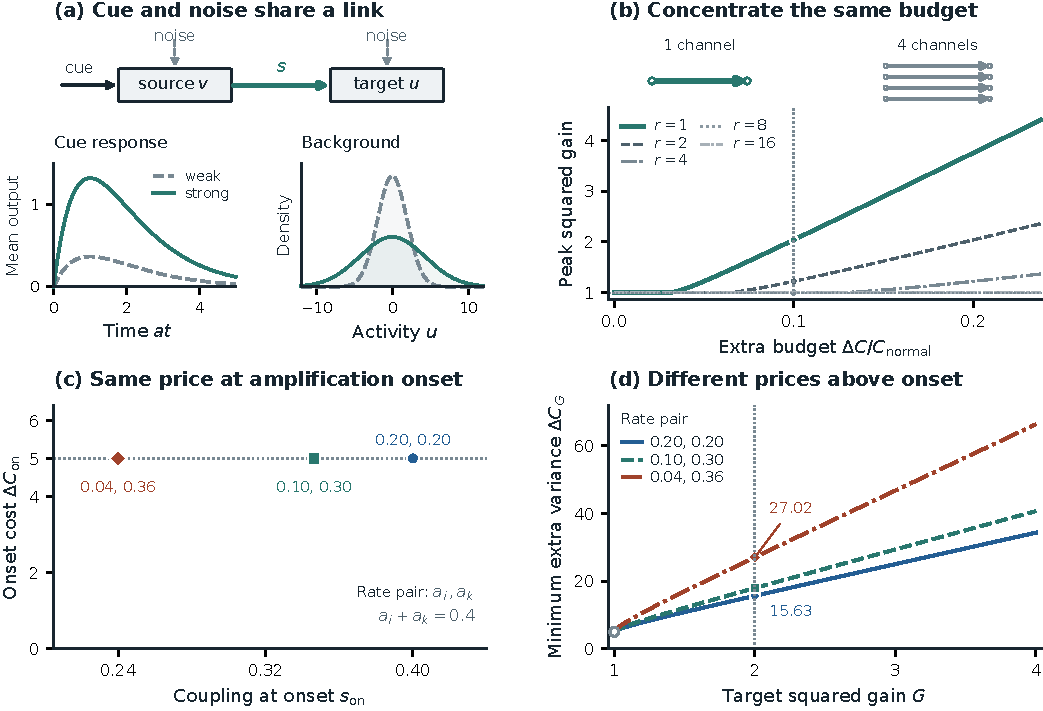
\includegraphics[width=\textwidth]{figures/fig_prr1_cost.pdf}
  \caption{\textbf{The cost of amplifying a perturbation.}
  (a) A unit cue and source noise reach target \(u\) through
  the same link \(s\); the target also receives independent noise.
  Both coordinates decay at \(a=0.2\). Lower plots compare the
  cue-evoked mean (left) and stationary activity density (right):
  stronger coupling raises the response but broadens the background.
  Gray dashed: \(s=0.2\); teal solid: \(s\simeq0.716\).
  (b) The same extra variance is shared among \(r\) equal,
  independent one-pass channels; the cartoons contrast one channel
  with four. Here \(N=64\), \(a=0.2\), and
  \(C_{\rm normal}=160\). The dotted line marks
  \(\Delta C/C_{\rm normal}=0.1\); points compare \(r=1,2,4\).
  A peak squared gain of one means no transient amplification.
  (c) Onset cost \(\Delta C_{\rm on}=2/(a_i+a_k)\) versus
  threshold coupling \(s_{\rm on}=2\sqrt{a_i a_k}\).
  The labeled rate pairs all have \(a_i+a_k=0.4\), hence cost
  five, despite different coupling thresholds. They share a rate
  sum, not a full spectrum.
  (d) Minimum extra variance for a target squared gain \(G>1\),
  using the same rate-pair colors and symbols as in (c).
  Points at \(G=2\) show the different prices above onset.
  The open point at \(G=1\) is the right-hand onset limit,
  not the cost of attaining unit gain.
  All panels use independent unit-intensity drive.}
  \label{fig:cost}
\end{figure}

\subsection{The price of a channel between two decay modes}

Now let two orthogonal coordinates have decay rates \(a_i,a_k>0\).
One directed coupling of strength \(m\) sends activity from \(k\)
to \(i\); no other coupling touches the pair. The two eigenvalues
remain \(-a_i\) and \(-a_k\) for any \(m\). With unit isotropic drive,
the coupling adds \(m^2/[2a_i a_k(a_i+a_k)]\) to the uncoupled variance
(Appendix~\ref{app:proof}). Amplification requires
\(m^2>4a_i a_k\), giving an onset cost of
\begin{equation}
  \Delta C_{\mathrm{on},ik}=\frac{2}{a_i+a_k}
  \label{eq:onset}
\end{equation}
Thus the product of the rates sets the required squared coupling,
but their sum sets the variance cost at onset
[Fig.~\ref{fig:cost}(c)].

Onset only tells us whether amplification is possible. For a
specified squared gain \(G>1\), we ask for the least extra variance
\(\Delta C_G\) that makes the pair's peak squared gain at least \(G\).
The transfer from an initial unit perturbation at \(k\) to coordinate
\(i\) is \(m f_{ik}(t)\), with
\(f_{ik}(t)=(e^{-a_k t}-e^{-a_i t})/(a_i-a_k)\) for \(a_i\ne a_k\),
and \(f_{ik}(t)=te^{-at}\) when \(a_i=a_k=a\).
The target \(G\) allows the best initial direction in the pair,
rather than fixing the cue to coordinate \(k\).
At each time the required coupling is obtained from the largest
singular value of the two-coordinate propagator. Minimizing its
variance cost over time gives
\begin{equation}
 \Delta C_G=\frac{1}{2a_i a_k(a_i+a_k)}
  \min_{t>0}\frac{(G-e^{-2a_i t})(G-e^{-2a_k t})}{G f_{ik}(t)^2}.
 \label{eq:targetcost}
\end{equation}
As \(G\) decreases to one, the cost approaches the onset value.
At finite gain, however, a common rate sum is not enough to fix
the cost. For example, the pairs \((0.20,0.20)\) and \((0.04,0.36)\)
both have onset cost \(5\), but reaching \(G=2\) costs \(15.63\)
and \(27.02\), respectively [Fig.~\ref{fig:cost}(d)].
For independent pairs that do not share coordinates, the costs add
and the largest pair gain sets the full system's gain. Therefore a
target \(G>1\) is reached most cheaply by coupling only the pair
with the lowest \(\Delta C_G\). This statement does not cover paths
that overlap or cooperate to amplify the same perturbation.

For a general stable real-eigenvalue spectrum, an orthogonal
change of coordinates puts \(J\) in real Schur form \(D+M\).
Here \(D\) is diagonal with entries \(-a_i\), and the strictly upper
triangular matrix \(M\) couples the coordinates without changing
those eigenvalues. For small \(\|M\|_F\), the excess variance above
the diagonal baseline is
\begin{equation}
  \Cnoise_I(J)-\sum_i \frac{1}{2a_i}
    =\sum_{i<k}\frac{M_{ik}^2}{2a_i a_k(a_i+a_k)}
      +O(\|M\|_F^3).
  \label{eq:weighted}
\end{equation}
Each coefficient is the time integral of \(f_{ik}(t)^2\).
The pair formula is exact at finite coupling because no longer
paths exist. With multiple paths this expansion describes only
weak coupling; it does not solve the general fixed-budget problem.

\subsection{Quieter inputs buy more directed response}

For a single equal-decay channel \(K=suv^\top\), let
\(q_v=v^\top Qv>0\) be the incoming noise intensity along its
source \(v\). If the drives at source and target are uncorrelated
(\(u^\top Qv=0\)), the excess cost is
\(\Delta C=s^2q_v/(4a^3)\) and the peak squared transfer from \(v\)
to \(u\) is \(s^2/(a^2e^2)\). Their ratio is
\begin{equation}
  \frac{\sup_t |u^\top e^{Jt}v|^2}
       {\Cnoise_Q(J)-\Tr Q/(2a)}
      =\frac{4a}{e^2 q_v}.
  \label{eq:anisotropic}
\end{equation}
For example, the assumption holds if \(v\) is an eigenvector of
\(Q\). A quieter source then allows stronger transfer for the same
extra variance. If the source and target drives are correlated,
the cost also contains a term linear in \(s\)
(Appendix~\ref{app:proof}). The comparison concerns the noise entering
the source, not the variance observed there after propagation.

Concentrating the budget maximizes peak response gain in the
equal-decay one-pass class. That objective does not yet specify
whether a selected output can distinguish the cue, because the
same coupling also amplifies background noise. We therefore next
fix the cue, output and integration window, and ask what the
expenditure buys for a downstream reader. Section~\ref{sec:allocation}
returns to allocation with this reliability objective in place.

\section{From gain-mediated routing to reliable readout}
\label{sec:window}

\subsection{Gain redistributes a fixed budget between outputs}

\begin{figure}[!t]
  \centering
  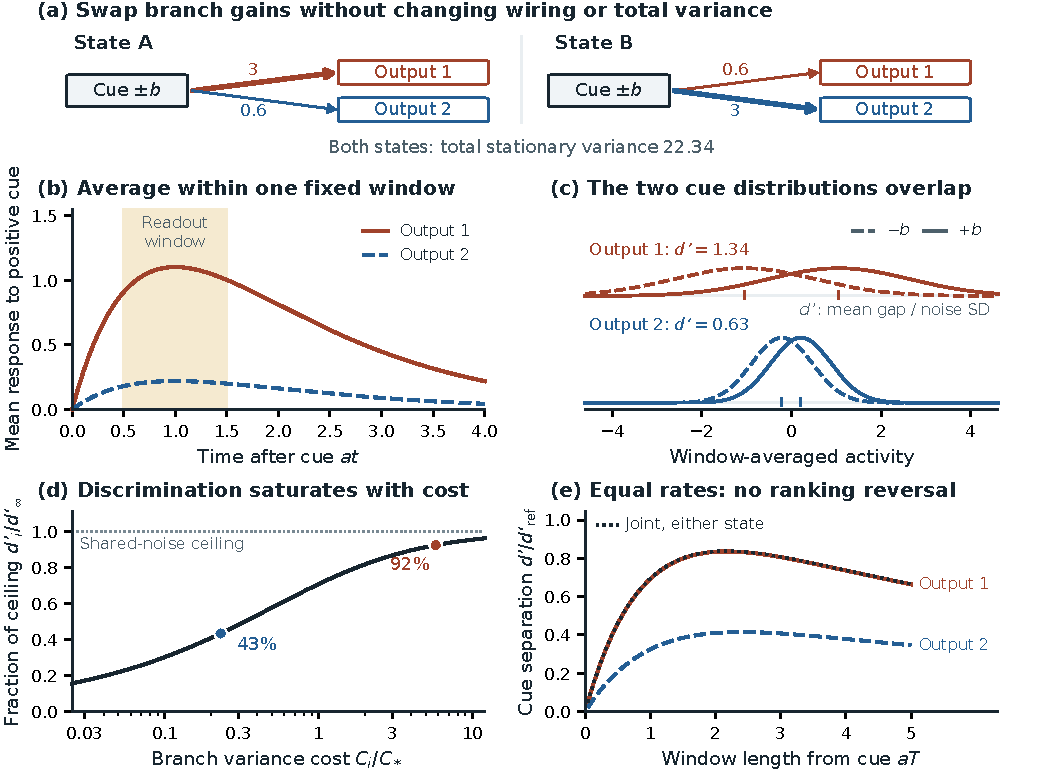
\includegraphics[width=\textwidth]{figures/fig_prr2_routing_polished.pdf}
  \caption{\textbf{Routing gains yield diminishing reliability returns.}
  (a) Both states receive one of the same two cues, \(\pm b\).
  Exchanging the gains \(3\) and \(0.6\) redistributes a fixed
  extra variance and switches the preferred output on unchanged
  wiring; total stationary variance remains \(22.34\).
  (b) Positive-cue mean responses in state A: output 1 is rust
  solid and output 2 blue dashed. Shading marks the window used
  in (c,d).
  (c) Gaussian distributions of the window averages for the
  two cues, with colors identifying outputs, dashed lines for
  \(-b\), and solid lines for \(+b\). The rows share a horizontal
  scale; vertical offsets only separate the densities.
  The stronger output has a fivefold larger cue-mean gap but a
  larger spread, so its \(d'\) is only about twice as large.
  (d) Each dot puts one branch on the cost law in
  Eq.~\eqref{eq:decodecost}, normalized by the cost \(C_*\)
  of reaching \(1/\sqrt{2}\) of the discrimination ceiling.
  State B exchanges the two dots between outputs.
  (e) Varying a window starting at cue onset changes \(d'\),
  but does not reverse the branch ranking in state A. The black
  dotted curve is the best joint readout, identical in both states.
  All curves use the same single-output reference ceiling from
  (d), not a duration-specific ceiling. This equal-timescale case
  is the control for Fig.~\ref{fig:crossover}.
  Model: \(N=40\), \(a=1\), \(Q=I\); the window in (b--d) is
  \(0.5\le at\le1.5\).}
  \label{fig:window}
\end{figure}

Figure~\ref{fig:window}(a) introduces the equal-timescale control: one
input feeds two fixed outputs on the same wiring, and gain
determines which output receives the larger response. The two
states allocate the same total fluctuation budget differently.
The gains are set before the cue and remain fixed during a trial.

The model has 40 units. Unit vectors \(b,c_1,c_2\) represent the
input and the two outputs and have disjoint support. The wiring
template \(W=(c_1+c_2)b^\top\) sends the input activity to both
outputs. In state \(s\), \(J_s=-aI+G_sW\), where the diagonal matrix
\(G_s\) scales incoming coupling at each unit but leaves the leak
\(a\) unchanged. The gains \(g=(g_1,g_2)^\top\) are \((3,0.6)^\top\)
in state A and \((0.6,3)^\top\) in state B; all other gains are one.
The effective coupling \(G_sW=(g_1c_1+g_2c_2)b^\top\) is one-pass
because neither output feeds the input (\(b^\top c_i=0\)).
This is why the eigenvalues stay fixed here; gain can shift
eigenvalues in a general recurrent circuit.

Equation~\eqref{eq:cost} gives the excess variance of output \(i\)
as \(C_i=g_i^2/(4a^3)\). Swapping the two gains redistributes
\(C_1+C_2\) without changing its value. With \(a=1\) the uncoupled
variance is \(20\) and both states have total cost \(22.34\).
Because the states are related by an orthogonal exchange of
outputs and the noise is isotropic, they also have identical
covariance eigenvalues and identical whole-state peak gain. The
fixed outputs are not exchanged by the observer: after a unit cue
along \(b\), output \(i\) still measures \(g_i t e^{-at}\).
The larger of the two signals therefore changes output identity.
This is a redistribution within a single input channel, not a
comparison between one and several independent channels.

\subsection{The budget price of cue discrimination}

Figure~\ref{fig:window}(b) shows the mean response after a positive
cue. The time variable \(at\) counts decay times \(1/a\), and the
favored mean is always five times larger. To assess whether the cue is
distinguishable, we start from stationary background activity
and apply one of two equally likely cues, \(\pm b\). Each readout
uses the average of \(c_i^\top x(t)\) in a common observation
window. The two states use the same cues, outputs, and window.

For a window starting at \(l\) with duration \(T\),
\(h=T^{-1}\int_l^{l+T}t e^{-at}\dd t\) is the mean signal per unit
branch gain for the positive cue. The two cue means are \(\pm hg\).
The covariance of the two averages is \(V_0 I_2+V_1 gg^\top\),
where \(V_0\) is the variance from noise entering each output
directly, and \(V_1\) is the variance per squared gain from noise
entering the common input. Both coefficients include correlations
over time (Appendix~\ref{app:window}). We quantify cue separation
by \(d'\), the difference between the two cue means divided by
their common standard deviation. For one output or the best linear
combination of both outputs in a known state, this gives
\begin{equation}
  d'_i=\frac{2hg_i}{\sqrt{V_0+V_1g_i^2}},\qquad
  d'_{\mathrm{joint}}=
  \frac{2h\|g\|_2}{\sqrt{V_0+V_1\|g\|_2^2}}.
  \label{eq:decode}
\end{equation}
The numerator of \(d'_i\) grows with \(g_i\), but so does the noise
in the denominator. Their ratio approaches the ceiling
\(d'_\infty(l,T)=2h/\sqrt{V_1}\) as \(g_i\) increases. With the
variance cost \(C_i\) defined above and
\(C_*=V_0/(4a^3V_1)\), the fraction of that ceiling and the cost
to reach a prescribed fraction \(\eta\in[0,1)\) are
\begin{equation}
 \left(\frac{d'_i}{d'_\infty}\right)^2=\frac{C_i}{C_i+C_*},
 \qquad C_i(\eta)=C_*\frac{\eta^2}{1-\eta^2}.
 \label{eq:decodecost}
\end{equation}
The scale \(C_*\) is the cost of reaching \(1/\sqrt{2}\) of the
discrimination ceiling, where shared input noise and direct drive
of the output contribute equally to the variance.
Equation~\eqref{eq:decodecost} turns a fluctuation constraint into
a quantitative allocation rule for the chosen readout. Improving
a favored output has diminishing returns: approaching its ceiling
requires an increasingly large share of the budget. At fixed
\(C_1+C_2\), moving cost toward one output improves its
discrimination at the expense of the other.
The optimal joint \(d'\) is unchanged because it depends only on
\(\|g\|_2=\sqrt{g_1^2+g_2^2}\). This is a benchmark that may use
a different combination of outputs in each state; it is not a
claim about a fixed downstream decoder or information transfer
for arbitrary cues.

Figure~\ref{fig:window}(c) shows the two cue distributions in the
reference window \(0.5\le at\le1.5\). The stronger branch spreads
their means farther apart but also broadens each distribution.
The fivefold mean contrast therefore becomes only about a
twofold contrast in \(d'\). The favored and other outputs
reach \(92\%\) and \(43\%\) of the same ceiling, as shown by
their positions on the cost curve [Fig.~\ref{fig:window}(d)].
In the later window
\(2\le at\le3\), the fractions are unchanged, but the ceiling itself
is smaller: the window has the same duration and noise variance,
yet captures a weaker signal. Figure~\ref{fig:window}(e) varies the
duration starting at cue onset and divides every score by the
single-output ceiling of the reference window. Averaging first
helps collect the cue; including too much of the decayed response
then reduces its separation.

\subsection{Output timescales change the value of an allocation}
\label{sec:crossover}

Figure~\ref{fig:window} changes the preferred output by swapping
gains; its equal output timescales keep the discrimination ranking
unchanged as the window varies. We now hold the gains fixed and
ask whether unequal output timescales can change that ranking.
To keep the two mean-response waveforms proportional, we use
two separate source--output pairs driven by the same cue,
rather than two branches of a common source
[Fig.~\ref{fig:crossover}(a)]. Each pair has only forward
coupling and independent unit-intensity white drive. One runs
from a fast source to a slow output; the other runs from a slow
source to a fast output. The same two rates
\(a_{\rm s}<a_{\rm f}\) occur in each pair. A positive cue shifts
both sources by \(1/\sqrt{2}\), and a negative cue shifts them
by the opposite amount. The output of each route is read
separately. The coupling to the slow output is \(m_{\rm s}\),
and that to the fast output is \(m_{\rm f}\), with
\(\gamma=m_{\rm s}/m_{\rm f}>1\).

The response kernel \(f_{ik}(t)\) in Sec.~\ref{sec:law} is
unchanged by interchanging its two rates. Thus the mean
response of the stronger route is larger by \(\gamma\) at
every \(t>0\) [Fig.~\ref{fig:crossover}(b)]. The propagated
source noise is also filtered by this same kernel and its
variance is proportional to \(m_i^2\). But noise entering
the output directly is filtered only by the output's own
decay rate. For an average over \([0,T]\), this local noise
has variance
\begin{equation}
 V_0(a,T)=\frac{aT-1+e^{-aT}}{a^3T^2},
 \qquad
 d'_i(T)=\frac{2m_i h(T)}
  {\sqrt{V_0(a_i,T)+m_i^2 V_1(T)}} .
 \label{eq:crossnoise}
\end{equation}
Here \(i\) denotes the slow or fast output, \(h(T)\) is the
positive-cue mean per unit coupling, and \(V_1(T)\) is the
window variance from source noise per squared coupling.
Both \(h\) and \(V_1\) are common to the two routes.

We can now express the comparison in the same budget units
as Sec.~\ref{sec:law}. Write
\(\kappa=[2a_{\rm s}a_{\rm f}(a_{\rm s}+a_{\rm f})]^{-1}\).
The allocated excess variance is \(\Delta C_i=\kappa m_i^2\).
Varying that pair's forward coupling and inverting
Eq.~\eqref{eq:crossnoise}, the least budget needed for output
\(i\) to attain a specified separation \(d>0\) is
\begin{equation}
 \Delta C_i(d,T)=
 \frac{\kappa\,d^2 V_0(a_i,T)}{4h(T)^2-d^2 V_1(T)},
 \qquad d<d'_\infty(T)=\frac{2h(T)}{\sqrt{V_1(T)}}.
 \label{eq:reliabilitycost}
\end{equation}
The two routes have identical response kernels and a common
discrimination ceiling, but different prices for reaching the
same reliability. For any target attainable by both at the
chosen window, their required budgets have ratio
\(V_0(a_{\rm s},T)/V_0(a_{\rm f},T)\), independent of the
target \(d\). This is an exact readout-cost relation within
the two-pair model, obtained by inverting the discrimination
formula and substituting the pair's variance cost. The fast
output is always cheaper at equal discrimination; the question
is whether the larger budget assigned to the slow output
compensates for this difference.

The actual allocation ratio is
\(\Delta C_{\rm s}/\Delta C_{\rm f}=\gamma^2\).
The stronger route is easier to read only if its budget advantage
outweighs its extra noise cost. In ratios, the condition is
\begin{equation}
 \gamma^2>\frac{V_0(a_{\rm s},T)}{V_0(a_{\rm f},T)}.
 \label{eq:crossover}
\end{equation}
The price ratio on the right grows strictly from \(R=a_{\rm f}/a_{\rm s}\)
to \(R^2\) as \(T\) increases from zero to infinity (Supplemental
Material~\cite{prrSupplement}). Short windows retain nearly all of
the local variance, proportional to \(1/a_i\); long windows also
reflect how long the fluctuations persist, giving a variance
proportional to \(1/(a_i^2T)\). For \(\sqrt R<\gamma<R\) there
is exactly one crossover. The slow output is better before it,
and the fast output afterward, despite its smaller mean signal.
The source-noise terms cancel from this ranking comparison.
Removing local noise ties the two \(d'\) curves; retaining only
local noise leaves the crossover unchanged. The mechanism is
therefore the window-dependent price of local fluctuations,
not just saturation from amplified source noise.

\begin{figure}[!t]
  \centering
  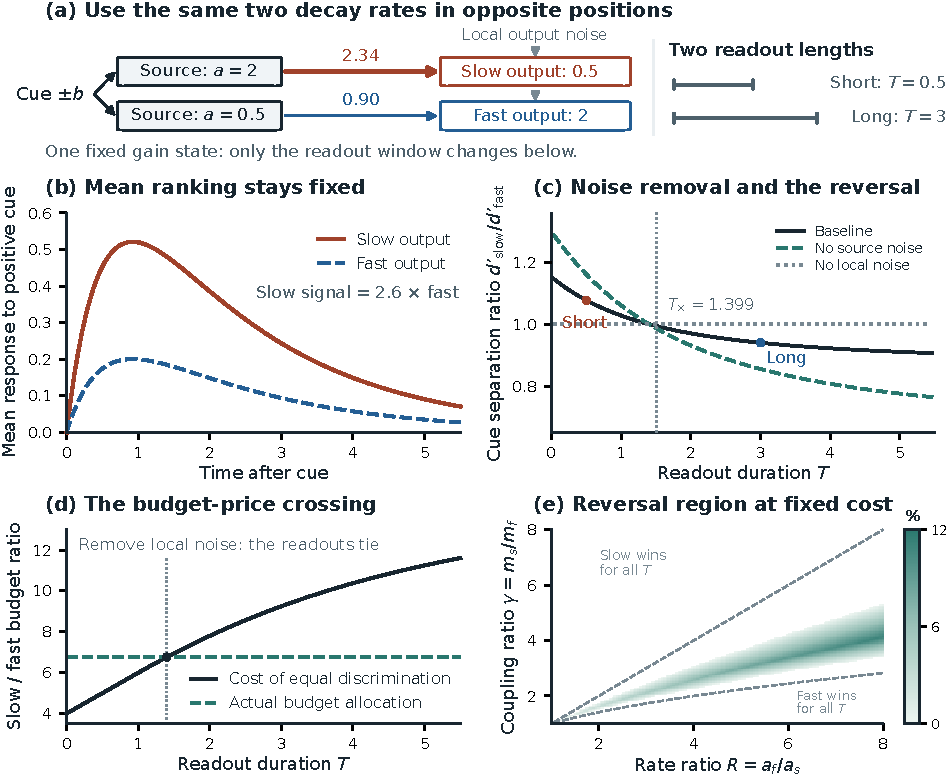
\includegraphics[width=\textwidth]{figures/fig_prr3_strengthened.pdf}
  \caption{\textbf{The stronger signal can be the worse readout.}
  (a) Unlike the common-source model of Fig.~\ref{fig:window},
  these routes have separate sources receiving the same cue,
  which shifts each source by \(\pm1/\sqrt{2}\).
  Each contains one fast and one slow coordinate, in opposite
  positions. Rust denotes the slow output and blue the fast
  output. Dashed arrows identify local output noise; the sources
  also receive independent noise. Gains remain fixed: only the
  readout window changes in (b--d).
  (b) A positive cue produces a \(2.6\)-fold larger mean response
  in the slow output (solid) than in the fast output (dashed)
  at every positive time.
  (c) Cue-separation ratios for the baseline (dark solid), removal
  of source noise (teal dashed), and removal of local output noise
  (gray dotted). The first two cross at \(T_\times=1.399\);
  removing local noise ties the readouts. Points mark the baseline
  at \(T=0.5\) (rust) and \(T=3\) (blue).
  (d) The dark curve is the ratio of budgets required for equal
  discrimination; it overtakes the actual allocation ratio
  \(6.76\) (teal dashed). By
  Eq.~\eqref{eq:reliabilitycost} this price ratio equals the
  ratio of local output noise variances. Panels (a--d) use rates \(0.5,2\),
  couplings \(2.34,0.90\), and independent unit white drive.
  Times are in model units, with \(\sqrt{a_{\rm s}a_{\rm f}}=1\);
  no conversion to physiological time is assumed.
  Noise interventions in (c) keep couplings, not variance cost, fixed.
  (e) Reversal region at fixed excess cost \(1.25712\), with
  \(a_s a_f=1\). Dashed boundaries \(\gamma=\sqrt R\) and
  \(\gamma=R\) delimit eventual reversal. Color gives the
  smaller fractional winning margin at the two specified windows,
  \(100\min[d_s'(0.5)/d_f'(0.5)-1,\,1-d_s'(3)/d_f'(3)]\),
  only where both margins are positive. White within the boundaries
  can have a crossing outside those windows. The open circle is
  the example in (a--d). Return-coupling, colored-noise and window-shape
  sensitivity checks are retained in the Supplemental Material.}
  \label{fig:crossover}
\end{figure}

For \(a_{\rm s}=0.5\), \(a_{\rm f}=2\) and
\((m_{\rm s},m_{\rm f})=(2.34,0.90)\), the stronger signal is
\(2.6\) times larger at every positive time. At \(T=0.5\) its
\(d'\) is \(0.394\) versus \(0.366\); at \(T=3\) it is \(0.638\)
versus \(0.679\). The crossing at \(T_\times=1.399\) is predicted
by the local noise ratio, not fitted to the \(d'\) curves
[Fig.~\ref{fig:crossover}(c,d)]. The reversal occurs within one
fixed gain state, without changing the wiring or switching routes.

Figure~\ref{fig:crossover}(c) directly tests the noise separation:
removing propagated source noise changes the ratios but not the
crossing, whereas removing local noise eliminates the ranking
difference. The effect occupies a finite region of parameters,
not an isolated point. Scanning rate and coupling ratios at fixed
excess cost and fixed \(a_s a_f=1\) gives the region in
Fig.~\ref{fig:crossover}(e). The analytic boundaries describe an
eventual crossing; the colored subset additionally requires opposite
rankings at the selected durations \(0.5\) and \(3\).

We test whether the reversal survives changes to the model
using fixed short and long effective durations \(0.5\) and \(3\).
We add weak return coupling from output to source, replace
white input by exponentially correlated noise of the same
integrated intensity, and use front-weighted triangular or
exponential readouts in addition to boxcar averages.
The Supplemental Material shows individual changes and an
example where combined changes remove the reversal at those
durations. With equal return couplings on both routes, \(65/75\)
tested combinations retain the reversal at the fixed durations.
These include all paired cases with noise correlation time at most
one quarter of the fast decay time. A separate gain-swap check
still matches decay and covariance spectra, total variance and
peak gain between states (Supplemental Material). When only one
route has a return coupling, \(48/60\) combinations retain the
reversal, but that gain-swap matching no longer holds exactly.
In all tested cases the stronger branch
still has a larger mean at both durations. For seven of the
22 cases that fail the fixed-duration test, the crossing
occurs before the short duration. These counts describe the
specified parameter grid; the exact crossing criterion above
applies to the white-noise, no-return model.

These comparisons use prescribed temporal weights. A covariance-optimal
linear readout of the sampled baseline trajectories removes the
reversal over \(0.15\le T\le5\). Uniform and signal-matched
weights retain it (Supplemental Material). The effect therefore
concerns a receiver's integration rule, not all accessible cue information.

\FloatBarrier
\section{Noise timescales and tasks determine routing allocation}
\label{sec:allocation}

The two-pair example isolates the role of local noise. We now allow
stable recurrence within each source and output population while
keeping the adjustable coupling between them one-way. The resulting
readout-cost law determines how to divide a budget among candidate
routes. We consider separately read outputs that must all remain
reliable, then a receiver that combines outputs for a joint cue
estimate.

\subsection{An exact readout-cost law for recurrent modules}

Let each pathway have a source population \(u_i\) and an output
population \(v_i\):
\begin{equation}
 \begin{aligned}
 \dd u_i&=A_i u_i\,\dd t+Q_{s,i}^{1/2}\dd W_{s,i},\\
 \dd v_i&=(D_i v_i+m_i B_i u_i)\,\dd t
                         +Q_{o,i}^{1/2}\dd W_{o,i}.
 \end{aligned}
 \label{eq:modules}
\end{equation}
Both internal matrices are stable and may contain recurrent,
non-normal dynamics. Only the coupling between populations is
unidirectional [Fig.~\ref{fig:allocation}(a)]. Its nonnegative
strength \(m_i\) is adjustable, while \(A_i,D_i,B_i\) and the
independent source and output drives are held fixed. The block
triangular generator keeps its eigenvalues for every \(m_i\).
Because output-local and propagated source fluctuations are
independent, the cost above the \(m_i=0\) baseline is exactly
\(x_i=\kappa_i m_i^2\), where \(\kappa_i>0\) is the propagated
stationary variance at unit coupling. This is finite-amplitude
pricing, not a weak-coupling expansion.

Apply opposite source cues and read a fixed scalar output with
a prescribed temporal weight. Let \(h_i(T)\) be its positive-cue
mean per unit coupling, \(L_i(T)>0\) its local-noise variance,
and \(S_i(T)>0\) its propagated variance per squared coupling.
We consider informative readouts with \(h_i(T)\ne0\).
Their exact combination is
\begin{equation}
 d_i'^2(x_i,T)=F_i(T)\frac{x_i}{x_i+C_{*,i}(T)},\qquad
 F_i=\frac{4h_i^2}{S_i},\quad
 C_{*,i}=\frac{\kappa_i L_i}{S_i}.
 \label{eq:modularlaw}
\end{equation}
Here \(F_i\) is the squared discrimination ceiling, while
\(C_{*,i}\) is the cost of reaching half of that squared ceiling.
Thus a pathway's dynamics and reader enter the allocation problem
through two quantities: its attainable reliability and the price
of approaching it. Equation~\eqref{eq:decodecost} is the
equal-rate common-source instance of this law. Matrix-exponential,
Lyapunov and quadrature calculations confirm it in 24 recurrent
module examples of total dimension 4--10 (Supplemental Material).

\subsection{A reversal criterion from noise timescales}

The ranking criterion also extends beyond Ornstein--Uhlenbeck
(OU) output noise.
For two pathways with the same \(h(T),S(T),\kappa\),
\(d_1'>d_2'\) precisely when \(x_1/x_2>L_1(T)/L_2(T)\).
Let \(R_i(\tau)\) be the autocovariance of the local output
fluctuations, and set \(P_i(0)=\int_{-\infty}^{\infty}R_i(\tau)\dd\tau\).
For a normalized nonnegative window \(w_T(t)=w(t/T)/T\),
short readouts retain \(L_i\to R_i(0)\), whereas long ones have
\(T L_i\to P_i(0)\int w^2\). If the covariances are continuous
at zero and absolutely integrable, with positive zero-frequency
power, then
\begin{equation}
 \frac{R_1(0)}{R_2(0)}<\frac{x_1}{x_2}
                 <\frac{P_1(0)}{P_2(0)}
 \label{eq:spectralreversal}
\end{equation}
guarantees at least one ranking reversal for continuously scaled
windows with nonzero common signal. The reverse ordering of
endpoints gives the opposite reversal. The window is assumed
integrable and square-integrable. OU mixtures and a damped
oscillatory component illustrate this prediction, alongside a
no-reversal control [Fig.~\ref{fig:allocation}(b)]. For OU noise
the endpoint ratios recover \(R\) and \(R^2\) in
Eq.~\eqref{eq:crossover}; uniqueness there follows from the
additional boxcar monotonicity, not from the endpoint test alone.
The required covariance is that of the local component, not the
unseparated total spontaneous activity.

The shared signal, propagated-noise and price coefficients matter.
Increasing only one source-noise intensity fourfold, while retaining
the baseline budget ratio, produces an example with no crossing
over the tested durations. The local-noise endpoints alone would
misclassify it if applied without checking those matching conditions.
The individual readout-cost law remains valid, but its unequal
ceilings and prices must be used (Supplemental Material).

\begin{figure}[p]
 \centering
 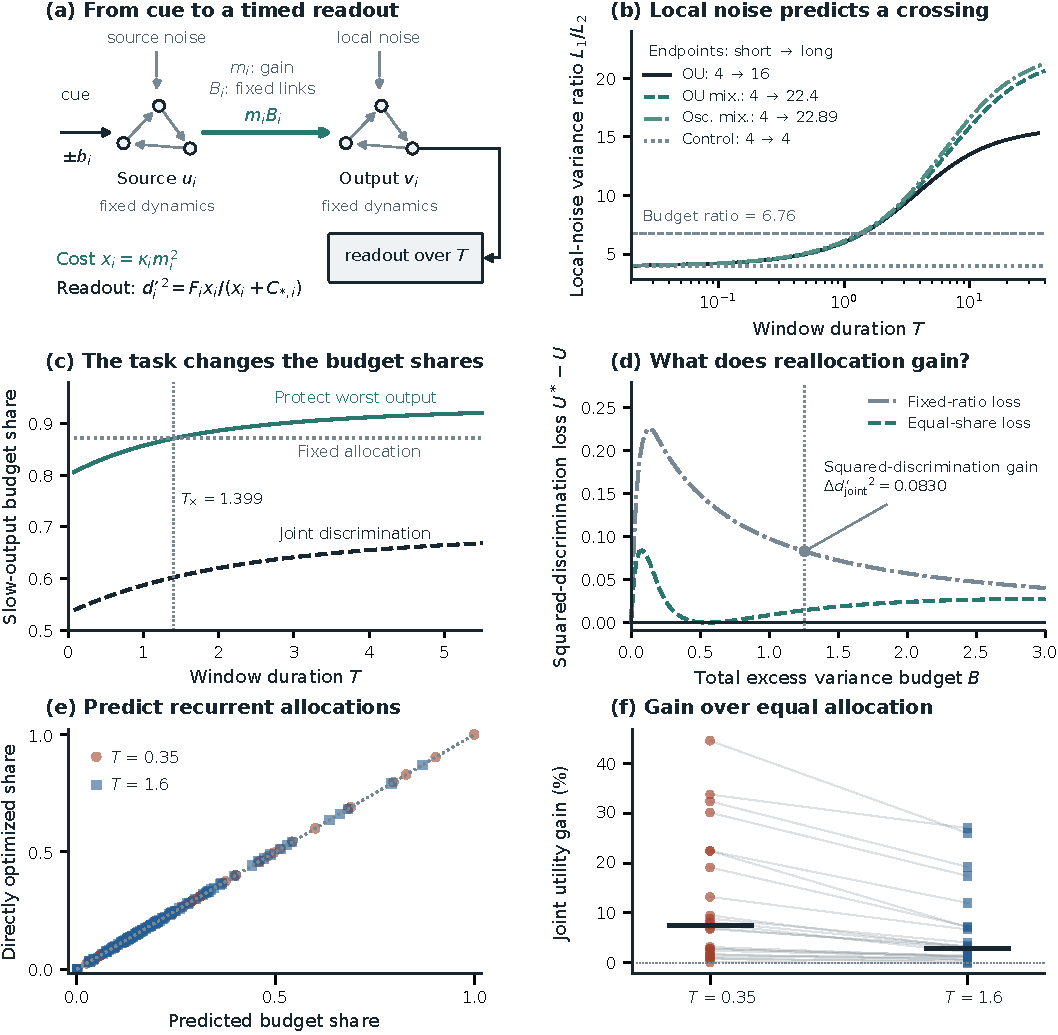
\includegraphics[width=\textwidth]{figures/fig_prr4_strengthened.pdf}
 \caption{\textbf{Noise timescales and task objectives set routing allocation.}
 (a) Cue \(\pm b_i\) reaches output \(v_i\) from source \(u_i\)
 through adjustable gain \(m_i\) on fixed links \(B_i\).
 Stable internal dynamics and independent drives give
 \(x_i=\kappa_i m_i^2\). Here \(F_i\) is the squared-discrimination
 ceiling and \(C_{*,i}\) the cost of reaching half that ceiling.
 (b) Local-noise variance ratios for illustrative covariances
 sharing signal and propagated-noise terms. Legend entries give
 short- and long-window endpoints; the dashed budget ratio is
 \(6.76\). OU denotes Ornstein--Uhlenbeck noise; the dotted control
 stays at four. These examples do not estimate prevalence.
 (c) Slow-output budget shares \(x_{\rm slow}/B\) at \(B=1.25712\): teal solid
 maximizes the worst separately read output, dark dashed maximizes
 joint discrimination, and gray dotted retains the fixed allocation.
 The first meets the fixed share at \(T_\times=1.399\).
 (d) Joint squared-discrimination loss \(U^*-U\) at \(T=3\),
 with \(U=d_{\rm joint}'^2\) and \(U^*\) its optimal value:
 gray dash-dot denotes the fixed ratio and teal dashed equal shares,
 each compared with the optimum at the same total budget \(B\).
 Zero marks the optimum reference. At the marked budget,
 reallocation raises joint \(d'\) from \(0.931\) to \(0.975\):
 \(0.0830\) in squared discrimination, not accuracy.
 Panels (c,d) use Fig.~\ref{fig:crossover}'s rates, cue and drive.
 (e) Predicted versus directly optimized joint budget shares in
 eight networks with \(2,4,6,8\) recurrent pathways, two windows
 and three budgets: 48 settings in total. Rust circles denote
 \(T=0.35\), blue squares \(T=1.6\); the dotted line is equality.
 (f) Joint-utility improvement over equal shares,
 \(100(U^*-U_{\rm equal})/U_{\rm equal}\), in those settings;
 lines pair the same network and budget across windows, and black
 bars denote medians. These are synthetic model settings, not
 independent biological samples.}
 \label{fig:allocation}
\end{figure}

\subsection{From a ranking reversal to a budget decision}

Suppose each output is needed by a separate downstream receiver.
Which reallocation improves the worst readout? For independent
pathways with budget \(\sum_i x_i\le B\), \(B>0\), and a common
ceiling \(F>0\), maximizing \(\min_i d_i'^2\) gives
\begin{equation}
 x_i^{\rm fair}=B\frac{C_{*,i}}{\sum_j C_{*,j}},\qquad
 \max\min_i d_i'^2=F\frac{B}{B+\sum_j C_{*,j}}.
 \label{eq:fairallocation}
\end{equation}
The optimum equalizes reliability by compensating each output's
price. For two pathways, equality of the discriminations is
equivalent to this max--min optimum. The physical consequence
comes from how the equalizing budget ratio changes with the
integration window, as local noise persists for different times.

With the existing example's fixed budget \(B=1.25712\), the
slow output receives \(1.09512\). The max--min optimum instead
assigns it \(1.0480\) at \(T=0.5\) and \(1.1345\) at \(T=3\),
meeting the fixed allocation at the ranking crossover \(T_\times=1.399\)
[Fig.~\ref{fig:allocation}(c)]. Before the crossing, reliability
of the worse output improves by moving budget from slow to fast;
after it, the improving transfer runs from fast to slow. Thus
Fig.~\ref{fig:crossover}'s fixed-state ranking predicts the
direction of useful compensation, not only which output wins.

Now let one receiver combine the independent scalar averages to
estimate the same cue. Then \(d_{\rm joint}'^2=\sum_i d_i'^2\).
More generally, fixed task weights \(p_i>0\) define the utility
\(U=\sum_i p_i d_i'^2\). Equation~\eqref{eq:modularlaw} is
strictly concave in each allocation. Its unique optimum is
\begin{equation}
 x_i^{\rm joint}=
 \left[\sqrt{\frac{p_i F_i C_{*,i}}{\lambda}}-C_{*,i}\right]_+,
 \qquad \sum_i x_i^{\rm joint}=B.
 \label{eq:allocationrule}
\end{equation}
Here \([z]_+=\max(z,0)\); the multiplier \(\lambda>0\) enforces
the budget and equalizes the weighted marginal benefit among
funded pathways. This is standard concave
resource allocation~\cite{boyd2004convex}; the physical inputs
here are the prices and ceilings derived from the dynamics.
The unweighted utility is joint discrimination only for independent
output noise, unlike the shared-source model in Fig.~\ref{fig:window}.
This task gives different slow-output budgets,
\(0.7088\) and \(0.8064\) at the two durations. At \(T=3\) it
raises joint \(d'\) from \(0.931\) to \(0.975\) at the same
cost. Figure~\ref{fig:allocation}(d) shows the squared-discrimination
regret \(\Delta U=U^*-U\): the fixed ratio leaves \(0.0830\)
unrealized at \(B=1.25712\), while equal shares are already close
to optimal for these parameters. Numerical constrained
optimization independently checks the allocation rule for
2, 4 and 8 pathways. The result is a readout-specific budget
frontier, not a rule that the strongest or currently most
reliable pathway should receive everything.

\subsection{Predicting allocations in heterogeneous recurrent pathways}
\label{sec:recurrentprediction}

We predict allocations from independently computed module
coefficients, without fitting performance curves across gains.
Eight fixed networks contain \(2,4,6,8\) pathways, with 40 pathways
in total and dense stable internal recurrence. Unit-gain quadrature
determines \(F_i(T)\) and \(C_{*,i}(T)\) before optimizing gains.
For windows \(0.35,1.6\) and three total budgets held fixed across
the windows, Eqs.~\eqref{eq:fairallocation}--\eqref{eq:allocationrule}
predict the allocations; unequal-ceiling max--min solutions use
the scalar target equation in the Supplemental Material.
We compare them against direct constrained optimization of
full-state means and covariances, without using the rational
readout law in that numerical objective.

Across the 48 network--window--budget settings, the largest
joint-allocation share discrepancy is \(7.1\times10^{-7}\)
[Fig.~\ref{fig:allocation}(e)]. Relative objective discrepancies
are below \(2.5\times10^{-13}\) for joint decoding and
\(2.4\times10^{-11}\) for max--min decoding. Joint utility gains
over equal shares range from \(0.0067\%\) to \(44.6\%\), with
median \(3.31\%\) [Fig.~\ref{fig:allocation}(f)]; thus some equal
allocations are already nearly optimal. Changing only the window
shifts the optimal joint budget shares by a median total variation
of \(0.101\), where total variation is half the sum of absolute
share changes. These checks demonstrate readout-specific
prediction on fixed recurrent circuits, not a biological
prevalence estimate. The heterogeneous pathways need not satisfy
the shared-term assumptions of the reversal criterion; their
individual cost laws still determine the allocation problem.

\subsection{Finding the allocation from performance feedback}

Can the weaker output be protected without specifying optimal
gains in advance? Consider a controller that redistributes a fixed
excess-variance budget \(B\) between trials. The model converts
each budget share into a coupling gain using its calibrated cost
coefficient \(\kappa_i\).
For equiprobable cues with symmetric Gaussian readouts, let \(\pi_i(x_i,T)\) be
the probability of a correct decision at output \(i\), using the
same prescribed temporal readout. It increases strictly with that
output's squared discrimination. An allocator can therefore give
budget to outputs that make more errors:
\begin{equation}
  \dot x_i=\eta[\bar\pi-\pi_i(x_i,T)],\qquad
  \bar\pi=\frac{1}{n}\sum_{j=1}^{n}\pi_j(x_j,T).
  \label{eq:feedback}
\end{equation}
Here \(n\) counts separately required outputs and \(\eta>0\)
sets the adaptation rate. With positive discrimination ceilings
and noise prices, this rule conserves \(B\), keeps budgets nonnegative,
and converges from any feasible allocation to the unique max--min
solution (Supplemental Material).
It needs comparable correctness feedback and a shared budget
pool, not the noise statistics or the target allocation.

In the two-pathway example, we replace the true probabilities by
finite batches of binary decision feedback. From the same initial
slow-output share of \(0.871\), the median learned shares are
\(0.830\) and \(0.900\) at the short and long windows, respectively
(theory: \(0.834\) and \(0.902\)). Switching from the short to the
long window also increases the learned share. These results use
\(131{,}072\) simulated decisions per output and window; shorter
runs are noisier (Supplemental Material).

The same controller also approaches the max--min allocation in a
four-pathway network from Sec.~\ref{sec:recurrentprediction}, with stable
recurrence within its modules. From equal shares, after 2,048
decisions per output the median improvement in worst-output
correctness is \(0.55\) and \(1.39\) percentage points at the two
windows, against achievable gains of \(0.90\) and \(1.82\) points.
After 131,072 decisions, the median allocation errors are \(0.024\)
and \(0.012\) in total variation. The Supplemental Material shows
trajectories, tests from each budget vertex, and a chance-feedback
control. These tests show how task feedback can improve the weaker
readout before the budget is closely matched to the optimum.

The calibrated budget-to-gain map can be replaced by a local
actuator (Supplemental Material). Neighboring routes trade target
budgets \(b_i\) in opposite directions according to their correctness
difference. Symmetric exchanges on a connected graph conserve
\(\sum_i b_i=B\) and recover the max--min optimum when realized
costs track their targets. Each route estimates its cost coefficient
from the cue-free variance of the unit-gain source-driven filter
\(\dot r_i=D_i r_i+B_i u_i\) and adjusts its actual gain by
\(\dot m_i=\gamma(b_i-\hat\kappa_i m_i^2)\). Here \(\gamma>0\)
sets the actuator rate and \(\hat\kappa_i\) is the local estimate.
This update is nonsingular at zero gain. The interior equilibrium
is locally stable at finite actuator rates in the deterministic
mean model. Only target budgets are conserved during adaptation;
actual gain-implied costs can lag.

In simulations that carry background activity across trials and
gain changes, the two-route controller raises the slow-route cost
from \(0.826B\) to \(0.898B\) after the readout window increases
(median; targets \(0.834B\) and \(0.902B\)). A sparse chain of
regulators also approaches the target in both four-route windows,
but substantial allocation error remains for eight routes at the
short window, even with a well-tracked total cost. This is a model
of slow feedback adaptation, not rapid or unsupervised biological
gain selection.
\FloatBarrier

\section{Discussion}

The computational value of flexible routing depends on its receiver,
not only its response amplitude. Source noise limits the reliability
gained by amplification, while local output noise sets a
window-dependent price for approaching that limit. The controlled
comparison isolates the latter mechanism: mean responses remain
proportional, yet their reliability ranking changes. At the crossing
window of the common-ceiling example, the fixed allocation equals
the max--min optimum; improving the worse output on either side
requires opposite budget transfers. A joint receiver instead
balances marginal benefits. The recurrent-module predictions show
how the same cost law yields these task-specific decisions beyond
the two-coordinate example.

The pair and readout costs answer complementary questions: which
decay modes make a transient response affordable, and where does
that expenditure buy useful cue discrimination? Concentration
maximizes peak gain in the equal-decay one-pass class, but it need
not maximize reliability for a specified receiver. This distinction
gives the fluctuation-budget hypothesis a computational test: compare
the attained discrimination with the appropriate readout-specific
frontier, rather than judging a gain state by its largest response.

The target-gain cost and the controlled ranking reversal are
connected by an exact readout-cost relation, now extended to
stable recurrent modules and an allocation frontier tested by
predicting gains in heterogeneous recurrent circuits.
The contribution builds on, rather than replaces, theories of
non-normal amplification and temporal coding. In the input-encoding
problem of Baggio \emph{et al.}~\cite{baggio2020communication},
short and long transmission windows can favor opposite allocations
of input power across decay modes. Here the cue and incoming noise
are fixed. We predict how to redistribute the stationary variance
spent on coupling gains to improve a specified reader's discrimination.
Azizpour \emph{et al.} instead optimize the recurrent interaction
strength, and hence distance to criticality, for finite-time
input discrimination~\cite{azizpour2026finite}. Our comparison
keeps decay rates fixed: the changing decision is which available
pathway to reinforce under a propagated-variance budget, not how
close the system should operate to criticality.
Amplified input
noise already explains limited signal-to-noise benefits at the
transient peak~\cite{bondanelli2020}; temporal correlations explain
limited integration benefits in cortex~\cite{goris2018integration}
and optimal representation scales~\cite{ahmed2026temporal}.
Our comparison fixes the two mean signals to the same temporal
shape and separates local from propagated noise.
Their ranking reversal is instead predicted by a local-noise
price ratio, independent of the common propagated source-noise
term. The crossing therefore isolates a computational consequence
of noise location, rather than a change in the deterministic signal.
Its endpoint criterion compares instantaneous local variance with
zero-frequency noise power, not a special pair of OU time constants.
The concave allocation method itself is established optimization;
the new connection is how dynamical noise prices determine both
the ranking and the task-dependent direction of reallocation.

There is also a distinction between opening a route and reading
it. Transient synchrony can create transmission windows through
collective dynamics~\cite{palmigiano2017routing}. Our externally
driven fluctuations act within a gain state and set the reliability
of its output. The feedback model adds a separate, slower process:
it adjusts an established set of gains between trials in response
to downstream errors. The distributed version assigns distinct
roles to neighboring competition and local activity estimates;
neither mechanism selects a task or sets the total target budget.
It does not generate collective routing states.
In particular, balancing output error rates does not solve the
joint-decoding task, which requires comparing marginal benefits.

The exact allocation statements vary independent nonnegative forward
gains, with no additional gain caps and with internal dynamics and
temporal readout weights held fixed. The readout-cost law allows
stable recurrence within modules; the local-noise reversal test
additionally needs matching coefficients across the two routes.
The heterogeneous allocation tests do not validate an unrestricted
reversal rule. Cross-module feedback and shared noise between
pathways lead to different optimization problems. The reversal is a
property of the prescribed temporal readout, not an ordering of
the information accessible in a complete sampled trajectory.
The accompanying FlyWire, ALM, and Allen analyses illustrate
anatomical and recording contexts, not evidence for biological
budget optimization. In particular, trained normal controls remove
the consistent ALM advantage seen with random orientations, and
the small Allen prediction improvement is exploratory
(Supplemental Material~\cite{prrSupplement}).

An experimental test would first estimate local and propagated
noise separately, for instance by independently perturbing the
source and output populations. In a matched pair, the local
autocovariances determine the window-dependent noise ratio; its
crossing of the fixed budget ratio predicts where the ranking
changes. Held-out cue trials can test the predicted ranking on
either side without fitting discrimination curves. Failure to
reverse would challenge the model once the matching and readout
assumptions are verified. An additional test would redistribute
gain in opposite directions at the same total variance cost and
measure which adjustment improves the weaker readout. Neither
test alone would establish that the brain chooses that adjustment;
that requires tracking its own gain changes and the feedback that
drives them.
Flexible routing is computationally effective when the allocation
of response capacity matches the receiver's noise, integration time
and objective. Gain controls the relative transfer to different
outputs; those downstream requirements determine which transfers
are worth strengthening under a fixed fluctuation budget.

\section*{Data and code availability}
The ALM recordings~\cite{chen2021modularity} are available from
Zenodo record 6713616~\cite{chenli2022dataset}. FlyWire anatomy and the reference model are
distributed by their respective projects~\cite{dorkenwald2024,shiu2024};
the Allen recordings are publicly available~\cite{siegle2021visual}.
The accompanying source archive includes the analysis code, numerical
results and reproduction instructions for this manuscript version.
Third-party raw data are obtained from the cited releases.
The project repository is
\url{https://github.com/Mia9469/SSNN}.

\section*{Use of AI tools}
Under author direction, OpenAI Codex (GPT-5 and GPT-6), OpenAI
ChatGPT (July--August 2026 web version), and Anthropic Claude Code
(Opus 4.8 and Sonnet 5) assisted with code debugging and manuscript
analysis. Codex also assisted with analysis implementation, numerical
verification, figure generation and presentation of the derivations.
The authors directed the analyses, reviewed the reported results, and
are responsible for the manuscript's accuracy and interpretation.

\appendix

\section{Exact response and cost calculations}
\label{app:proof}

\subsection{Equal decay and one-pass coupling}

Since \(K^2=0\), the image of \(K\) lies in its kernel, so nonzero left
singular vectors \(u_i\) are orthogonal to the corresponding right
subspace spanned by the \(v_i\). In each plane \((u_i,v_i)\),
the propagator is \(e^{-at}\left(\begin{smallmatrix}1&ts_i\\0&1
\end{smallmatrix}\right)\). Its largest squared singular value is
\(e^{-2at}(\sqrt{1+(ts_i)^2/4}+ts_i/2)^2\), increasing in \(s_i\)
for any fixed \(t>0\). Directions in the orthogonal complement all
decay at rate \(a\). Thus above onset, when the optimum occurs at positive time,
concentrating \(\sum_i s_i^2\) in one channel maximizes
Eq.~\eqref{eq:peak}. The largest eigenvalue of the symmetric part
is \(-a+s_1/2\); squared Euclidean norm has derivative
\(x^\top(J+J^\top)x\). A nonpositive symmetric part gives contraction
at all times, and a positive direction gives immediate growth.

For isotropic drive \(\Cnoise_I=\int_0^\infty \|e^{Jt}\|_F^2\dd t\).
The integrand in the square-zero class is
\(e^{-2at}(N+t^2\|K\|_F^2)\) because \(\Tr K=0\), proving
Eq.~\eqref{eq:cost}. At \(s_1=2a\) the rank-one cost increment is
\(1/a\). For arbitrary \(Q\) and \(K=suv^\top\), the increment is
\(s\,u^\top Qv/(2a^2)+s^2 v^\top Qv/(4a^3)\).
The peak squared directed response from \(v\) to \(u\) is
\(s^2/(e^2a^2)\), which gives Eq.~\eqref{eq:anisotropic} under
its stated assumption.

\subsection{Unequal decay and isolated pairs}

For the Schur calculation, the first-order off-diagonal element of
\(e^{(D+M)t}\) is \(M_{ik}f_{ik}(t)\), with
\[
  f_{ik}(t)=\int_0^t e^{-a_i(t-u)}e^{-a_k u}\dd u .
\]
The diagonal stays equal to that of \(e^{Dt}\), and
\(\int_0^\infty f_{ik}^2\dd t=[2a_i a_k(a_i+a_k)]^{-1}\),
including the continuous equal-rate limit. Squaring the
off-diagonal contributions gives Eq.~\eqref{eq:weighted}.
With one nonzero \(M_{ik}\), all higher-order terms in the propagator
vanish. On this pair the symmetric part is negative semidefinite
exactly for \(m^2\le4a_i a_k\). The formula for the threshold cost
follows by substitution.

For the finite-gain law, the pair propagator at time \(t\) has
diagonal entries \(x=e^{-a_i t}\), \(y=e^{-a_k t}\) and upper
entry \(m f_{ik}(t)\). Its squared singular values are the
eigenvalues of \(P^\top P\), with \(P\) this propagator. Thus
\[
 \det(GI-P^\top P)=(G-x^2)(G-y^2)-Gm^2 f_{ik}(t)^2 .
\]
The smaller squared singular value is no larger than \(x^2<1\),
so for \(G>1\) the zero of this expression gives exactly the
coupling needed to attain \(G\) at \(t\). Minimizing over
positive \(t\) and converting coupling to excess cost gives
Eq.~\eqref{eq:targetcost}. The objective diverges at both time
endpoints for fixed \(G>1\), so the minimum is attained.
Any such coupling must exceed the onset threshold. Conversely,
as \(G=1+\epsilon\) tends to one, choosing
\(t=\sqrt{\epsilon}/(a_i+a_k)\) makes the required \(m^2\) tend to
\(4a_i a_k\). This gives the right-hand limit; attaining \(G=1\)
itself requires no excess cost.

\section{Window covariance in the two-output model}
\label{app:window}

The two-output stationary lag covariance at lag \(u\ge0\) is
\begin{equation}
  L(u)=e^{-au}\left(\frac{I_2}{2a}+
                      \frac{1+au}{4a^3}\,gg^\top\right).
\end{equation}
This is obtained by projecting \(e^{Ju}\Sigma\) to the two fixed output
directions, with \(J=J_s\) and \(\Sigma\) the stationary covariance in
the chosen state. The cue only shifts the mean of the linear Gaussian
process. For a window of length \(T\), the covariance of the averages
is \(2T^{-2}\int_0^T (T-u)L(u)\dd u\); \(V_0,V_1\) are the resulting
coefficients of \(I_2\) and \(gg^\top\).
This calculation accounts for noise shared by the two outputs and for
correlations over time. The equal-prior accuracy is \(\Phi(d'/2)\),
where \(\Phi\) is the standard Gaussian cumulative distribution.
The single-output readout uses a fixed zero threshold. The joint readout
is an upper benchmark for the two averages with state known, and may
use a different optimal direction in each state. Matrix-exponential
and Lyapunov calculations reproduce the mean and lag covariance used
in the scalar integrals.


\clearpage
\bibliographystyle{apsrev4-2}
\bibliography{references,references_prr}
\end{document}
